\documentclass[11pt,a4paper]{article}
\usepackage{kotex}
\usepackage{amsmath, amssymb, amsthm}
\usepackage{graphicx}
\usepackage{hyperref}
\usepackage{geometry}
\usepackage{listings}
\usepackage{xcolor}
\usepackage{setspace}

\geometry{margin=1.2in}
\setstretch{1.6} % 넉넉한 줄간격으로 분량 확보 및 가독성 향상

% 들여쓰기 및 문단 설정
\usepackage{indentfirst} % 첫 단락 들여쓰기 강제 적용
\setlength{\parindent}{1.5em} % 문단 들여쓰기를 1.5em으로 고정
\setlength{\parskip}{0pt} % 문단 간 격차는 0으로 유지하여 들여쓰기의 시각적 일관성 유지

% TikZ 그리기 패키지 로드
\usepackage{tikz}
\usetikzlibrary{shapes.geometric, arrows.meta, positioning, shadows, calc}

\definecolor{codegreen}{rgb}{0,0.6,0}
\definecolor{codegray}{rgb}{0.5,0.5,0.5}
\definecolor{codepurple}{rgb}{0.58,0,0.82}
\definecolor{backcolour}{rgb}{0.95,0.95,0.92}

\lstdefinestyle{mystyle}{
    backgroundcolor=\color{backcolour},   
    commentstyle=\color{codegreen},
    keywordstyle=\color{magenta},
    numberstyle=\tiny\color{codegray},
    stringstyle=\color{codepurple},
    basicstyle=\ttfamily\footnotesize,
    breakatwhitespace=false,         
    breaklines=true,                 
    captionpos=b,                    
    keepspaces=true,                 
    numbers=left,                    
    numbersep=5pt,                  
    showspaces=false,                
    showstringspaces=false,
    showtabs=false,                  
    tabsize=2
}
\lstset{style=mystyle}

\title{\Huge\textbf{OMI (Orchestrated Math Interpreter)} \\ \vspace{0.8cm} \Large 5단계 심층 추론 및 역공학 데이터셋 기반의 \\ 고도화된 AI 수학 튜터 시스템 종합 연구 보고서}
\author{\textbf{AIMO Project Research Team}}
\date{\today}

\begin{document}

\maketitle

\begin{abstract}
최근 자연어 처리(Natural Language Processing) 분야에서 대형 언어 모델(Large Language Models, LLMs)은 눈부신 발전을 이룩하며 인간의 언어 능력을 모방하는 데 성공했습니다. 텍스트 요약, 번역, 코드 작성 등 다양한 영역에서 상용화 수준의 성과를 보이고 있으나, 고도의 논리적 엄밀성과 다단계 계산이 요구되는 수학적 추론(Mathematical Reasoning) 영역에서는 여전히 치명적인 한계를 드러내고 있습니다. 모델이 텍스트를 생성할 때 발생하는 `환각(Hallucination)' 현상과 산술적 연산 능력의 부재는 복잡한 수식과 증명을 요구하는 문제에서 오답을 정당화하는 확증 편향(Confirmation Bias)으로 이어집니다.

본 연구는 이러한 LLM의 근본적인 한계를 극복하기 위해, AI가 인간 수학자의 사고 과정을 단계별로 모방할 수 있도록 설계된 \textbf{OMI (Orchestrated Math Interpreter)} 시스템을 제안합니다. 이 시스템은 AI가 머릿속으로 모든 것을 계산하게 두는 대신, 파이썬(Python) 코드와 같은 외부 도구를 적극적으로 활용할 수 있는 환경을 제공합니다. 

본 보고서에서는 시스템의 뼈대가 되는 \textbf{5단계 심층 추론 파이프라인(5-Stage Deep Reasoning Pipeline)}을 제안합니다. 이 파이프라인은 문제의 도메인을 분류하는 Labeling 단계부터, 필요한 수학적 지식을 불러오는 Retrieval, 문제 스케일에 따라 시뮬레이션과 이론적 해법을 결정하는 Router, 파이썬 샌드박스를 통해 실제 수식을 계산하는 Execution, 그리고 결과를 다각도로 검증하는 Verification 단계로 구성됩니다. 

또한, 단일 모델의 한계를 돌파하기 위해 다수결 투표(Majority Voting)와 다중 에이전트 토론(Multi-Agent Debate)이라는 앙상블 기법을 도입하여 수학적/물리적 무결성을 획기적으로 향상시켰습니다. 나아가 AI 모델의 추론 능력을 고도화하기 위한 학습 데이터의 오염 문제를 해결하고자, 정답으로부터 문제를 파생시키는 \textbf{역공학(Reverse Engineering) 기반의 데이터 생성 기법(Open-Reverse-Math)}을 최초로 고안 및 적용하였습니다.

최종적으로, 이 모든 복잡한 백엔드 아키텍처와 AI의 사고 과정을 일반 사용자와 학습자가 직관적으로 이해할 수 있도록 시각화한 `투명한 유리 상자(Glass-box)' 형태의 웹 대시보드를 구축하였습니다. 이를 통해 OMI 프로젝트가 단순한 질의응답 시스템을 넘어, 향후 논리와 추론이 필요한 모든 산업 및 교육 도메인으로 확장 가능한 차세대 Agentic AI의 표준 아키텍처임을 입증하고자 합니다.

\end{abstract}

\newpage
\tableofcontents
\newpage

\section{Introduction (서론)}

\subsection{연구의 배경: 대형 언어 모델의 시대와 그 이면}
2020년대 이후, Transformer 아키텍처에 기반한 대형 언어 모델(Large Language Models, 이하 LLM)은 기계 학습과 인공지능 역사상 유례없는 파급력을 보여주고 있습니다. GPT-4, Claude 3, Gemini, 그리고 오픈소스인 Qwen 및 Llama 시리즈에 이르기까지, 최신 모델들은 방대한 양의 텍스트 데이터를 섭취하여 인간의 언어를 능숙하게 구사하게 되었습니다. 이들은 문서를 요약하고, 창의적인 시를 작성하며, 프로그래밍 언어로 어플리케이션을 코딩하는 등 지식 노동의 상당 부분을 자동화하는 수준에 도달했습니다.

그러나 이러한 언어적 유창함의 이면에는 치명적인 약점이 존재합니다. 바로 `엄밀한 논리와 수학적 계산(Strict Logic and Mathematical Calculation)' 능력의 부재입니다. 일반적인 자연어 처리 작업과 달리 수학 문제는 단 한 번의 연산 실수나 논리적 비약이 최종 결과의 완전한 붕괴를 초래합니다. "12345와 67890을 곱하면 얼마인가?" 혹은 "$100!$ 의 끝에 연속된 $0$의 개수는 몇 개인가?"와 같은 질문에 대해, LLM은 정답이 아닌 '그럴듯한 오답'을 매우 자신감 있는 어조로 출력하는 현상, 즉 환각(Hallucination)을 빈번하게 발생시킵니다.

\subsection{AI는 왜 수학을 못하는가? (The Mathematical Bottleneck)}
LLM이 수학 문제에 취약한 원인은 모델의 근본적인 작동 방식에서 기인합니다. 

첫째, \textbf{자기 회귀(Auto-regressive) 특성으로 인한 에러 누적}입니다. LLM은 이전까지 생성된 토큰(단어의 조각)들을 바탕으로 바로 다음 토큰의 확률을 계산하여 텍스트를 이어나갑니다. 만약 추론의 첫 번째 단계에서 사소한 덧셈 실수를 저지르게 되면, 모델은 그 오답을 기정사실화하여 이후의 모든 논리를 그 오답에 맞춰 전개하게 됩니다. 이를 확증 편향(Confirmation Bias)이라 하며, 스스로 실수를 인지하고 되돌아가는 능력(Backtracking)이 부족하기 때문입니다.

둘째, \textbf{토크나이저(Tokenizer)의 한계}입니다. 언어 모델은 텍스트를 의미 단위로 쪼개어 인식하는데, 숫자의 경우 그 패턴이 불규칙하게 쪼개지곤 합니다. 예를 들어 '12345'라는 숫자가 '123'과 '45'로 분리되어 벡터 공간에 저장되면, 숫자의 자릿수와 물리적 크기에 대한 감각(Number Sense)이 상실됩니다. 이로 인해 모델은 숫자의 덧셈과 곱셈을 진정한 의미의 산술(Arithmetic)이 아닌 텍스트 패턴 매칭(Pattern Matching)으로 해결하려 시도하게 됩니다.

셋째, \textbf{작업 기억(Working Memory)의 부재}입니다. 인간은 복잡한 다단계 연산을 수행할 때 종이에 중간 결과를 적어두거나(Scratchpad), 외부의 계산기를 활용합니다. 반면 기본 상태의 LLM은 모든 연산을 오로지 신경망 내부의 파라미터 연산(머릿속 암산)만으로 해결해야 하는 가혹한 제약 조건 하에 놓여 있습니다.

\subsection{OMI (Orchestrated Math Interpreter) 제안: 발상의 전환}
본 연구는 "AI에게 머릿속으로만 계산하도록 강요하는 것이 옳은가?"라는 질문에서 출발했습니다. 인간 수학자가 어려운 문제를 풀 때 계산기를 사용하고 공학용 소프트웨어를 활용하듯, AI에게도 동일한 도구를 쥐여준다면 어떨까요?

이러한 철학을 바탕으로 개발된 \textbf{OMI (Orchestrated Math Interpreter)} 시스템은 AI의 역할을 단순히 '답을 뱉어내는 자'에서 '문제를 어떻게 풀지 계획하고, 필요한 도구를 사용해 답을 조립하는 지휘자(Orchestrator)'로 재정의합니다. OMI 시스템 내에서 LLM은 파이썬(Python)이라는 강력하고 결함 없는 산술 연산 엔진과 결합됩니다. AI는 자연어로 문제를 분석하여 해결 논리를 파이썬 코드로 작성하고, 샌드박스(Sandbox) 환경에서 코드를 실행하여 나온 정확한 결과값을 토대로 수학적 결론을 도출합니다. 

이를 통해 AI의 가장 큰 약점이었던 '연산 실수'를 파이썬 인터프리터가 원천 차단하고, AI는 본연의 강점인 '논리적 방향성 제시'와 '코드 작성'에만 집중할 수 있게 됩니다.

\subsection{주요 기여도 및 연구 성과 (Key Contributions)}
본 프로젝트는 단순히 파이썬을 붙이는 수준을 넘어, 수학 교육 및 풀이 시스템의 패러다임을 바꿀 수 있는 혁신적인 파이프라인과 데이터셋 생성 기법을 포함하고 있습니다. 주요 기여도는 다음과 같습니다.

\begin{enumerate}
    \item \textbf{5단계 심층 추론 파이프라인(5-Stage Deep Reasoning Pipeline) 구축:} 
    문제를 도메인별로 라벨링(Labeling)하고, 맞춤형 지식을 검색(Retrieval)하며, 문제 스케일에 따라 시뮬레이션 혹은 이론적 접근으로 경로를 나누는 라우팅(Routing), 그리고 안전한 파이썬 실행(Execution)과 축소 검증(Verification)으로 이어지는 총체적 워크플로우를 확립했습니다.
    
    \item \textbf{다중 에이전트 앙상블(Multi-Agent Ensemble) 기반의 무결성 확보:} 
    패스 앳 케이(Pass@k) 확률 모델을 활용한 다수결 투표(Majority Voting) 시스템과, Coder와 Reviewer 역할을 분리하여 AI의 확증 편향을 끊어내는 다중 에이전트 토론(Debate) 메커니즘을 도입하여 난제에 대한 정답률을 극대화했습니다.
    
    \item \textbf{역공학(Reverse Engineering) 기반의 무오류 합성 데이터 엔진:} 
    데이터 오염(Data Contamination)을 막고 완벽한 참(True)이 보장되는 고품질 훈련 데이터를 무한대로 생성하기 위해, 정답으로부터 수식을 역으로 파생시키고 이를 자연어 문제로 감추는(Obfuscation) 새로운 데이터 합성 기법(Open-Reverse-Math)을 제안합니다.
    
    \item \textbf{Glass-box 기반의 교육용 웹 대시보드 및 XAI 시각화:} 
    백엔드에서 벌어지는 복잡한 라우팅과 파이썬 실행 과정을 프론트엔드 대시보드(Vite+React)를 통해 실시간으로 렌더링합니다. 또한 XAI(Explainable AI) 기술을 통해 AI의 전략 선택 이유를 인간의 언어로 풀어내어 투명하고 신뢰할 수 있는 교육 시스템을 완성했습니다.
\end{enumerate}

\subsection{보고서의 구성 (Document Structure)}
본 보고서는 총 5개의 섹션으로 구성되어 있으며, 각각의 섹션은 OMI 시스템의 핵심 요소들을 심도 있게 다룹니다.
제 2장(Related Work)에서는 Tool-Integrated Reasoning과 다중 에이전트 시스템에 관한 학계의 기존 연구와 그 한계를 분석합니다.
제 3장(Methodology)에서는 본 연구의 핵심인 5단계 심층 추론 파이프라인의 알고리즘 원리와 수학적 증명, 그리고 역공학 데이터 생성 엔진의 상세 로직을 묘사합니다.
제 4장(System Implementation)에서는 Vertex AI 기반의 클라우드 아키텍처와 이를 시각화하는 대시보드의 실전 구동 시나리오를 다룹니다.
마지막으로 제 5장(Conclusion)에서는 본 프로젝트의 의의와 향후 확장성에 대해 논의하며, 부록(Appendix)을 통해 비전공자도 쉽게 이해할 수 있는 상세한 용어 사전을 제공합니다.

\newpage
\section{Related Work: AI는 왜 수학을 못할까? (관련 연구 및 배경)}

본 연구의 OMI 아키텍처는 인공지능 학계에서 활발하게 논의되고 있는 세 가지 거대한 흐름 위에 구축되었습니다. 첫째는 LLM에 외부 도구를 쥐여주는 도구 결합 추론(Tool-Integrated Reasoning), 둘째는 확률 모델을 활용하여 정답을 보정하는 앙상블 및 다수결 투표(Majority Voting), 셋째는 여러 모델이 역할을 나누어 상호작용하는 다중 에이전트 토론(Multi-Agent Debate) 시스템입니다. 본 장에서는 각 분야의 기존 연구 성과와 그 한계를 짚어보고, 본 연구가 어떠한 차별점을 가지는지 심도 있게 분석합니다.

\subsection{Tool-Integrated Reasoning (도구 결합 추론의 진화)}
대형 언어 모델 초기에는 "모든 지식을 파라미터 내부에 저장하고, 모든 연산을 신경망으로만 처리해야 한다"는 암묵적인 가정이 존재했습니다. 이로 인해 GPT-3 모델 등은 세 자리 수의 곱셈이나 사칙연산조차 제대로 수행하지 못하는 현상을 보였습니다. 그러나 이러한 접근법은 비효율적임이 입증되었습니다. 마치 인간이 머릿속으로 미적분 방정식을 암산하지 않고 종이와 펜, 혹은 계산기를 꺼내 드는 것과 같은 이치입니다.

\subsubsection{PAL (Program-Aided Language models) 과 PoT (Program of Thoughts)}
이러한 문제를 해결하기 위해 제시된 초기 연구가 바로 PAL(Gao et al., 2023)과 PoT(Chen et al., 2022)입니다. 기존의 Chain-of-Thought(CoT) 프롬프팅이 "문제를 한 단계씩 풀어서 자연어로 설명해봐"라고 명령했다면, PAL과 PoT는 "문제를 푸는 과정을 파이썬 코드로 작성하고 변수를 할당해봐"라고 명령합니다. 

예를 들어, "철수가 사과 3개를 가지고 있고, 영희가 5배를 주었다면 총 몇 개인가?"라는 문제에서 모델은 다음과 같은 코드를 생성합니다.
\begin{lstlisting}[language=Python, caption=Program-Aided Language Model 예시]
apples_cheolsu = 3
apples_given_by_younghee = apples_cheolsu * 5
total_apples = apples_cheolsu + apples_given_by_younghee
print(total_apples)
\end{lstlisting}
이렇게 작성된 코드는 백그라운드의 파이썬 인터프리터에서 실행되고, 모델은 출력된 `18`이라는 완벽한 결과값을 가져와 사용자에게 전달합니다. 이 방식은 LLM의 최대 약점인 '계산 오류'를 파이썬이라는 절대적으로 신뢰할 수 있는 외부 엔진(Symbolic Engine)으로 분리(Decoupling)시켰다는 점에서 혁명적이었습니다. 

\subsubsection{기존 TIR 연구의 한계와 OMI의 차별점}
그러나 기존 PAL이나 PoT 방식은 1차원적인 코드 실행에 그쳤습니다. 만약 작성한 파이썬 코드에 `SyntaxError`나 무한 루프(`Timeout`)가 발생하면 시스템은 그대로 정지해버리며 오답을 반환했습니다. 

반면 본 프로젝트의 OMI 파이프라인은 \textbf{실패를 전제로 한 반복적 수정(Iterative Refinement)} 구조를 갖추고 있습니다. Stage 4 (Execution) 단계에서 에러가 발생할 경우, 모델은 에러 추적 메시지(Traceback)를 읽고 "아, 숫자가 너무 커서 메모리 초과가 났구나. 수학 공식(Theoretician 접근)으로 다시 코드를 짜야겠다"라고 자가 교정(Self-Correction)을 수행합니다. 이는 단순한 도구 사용을 넘어선 진정한 의미의 '도구 결합형 에이전트'입니다.

\subsection{Ensemble Methods: Pass@$k$ 와 Majority Voting}
수학 문제는 본질적으로 정답이 하나로 수렴하는 독특한 특징을 가집니다. 일반적인 글쓰기나 번역은 수백 가지의 '좋은 답'이 존재할 수 있지만, 정수론이나 대수학 문제에서는 $x=42$ 라는 유일한 해답만이 존재합니다.

\subsubsection{Pass@$k$ 확률 모델의 수학적 원리}
언어 모델은 Temperature 매개변수가 0보다 클 때, 매번 다른 궤적을 그리며 텍스트를 생성합니다. 즉, 동일한 문제를 줘도 첫 번째 시도에는 중간에 덧셈을 틀리고, 두 번째 시도에는 올바르게 풀 수 있습니다. 어떤 모델이 한 번 시도했을 때 정답을 맞힐 확률(Pass@1)이 $p$라고 합시다. 만약 이 모델에게 독립적으로 $k$번 문제를 풀게 했을 때, 그 중 적어도 한 번은 올바른 풀이를 생성할 확률, 즉 Pass@$k$는 다음과 같이 정의됩니다.
\begin{equation}
Pass@k = 1 - (1 - p)^k
\end{equation}
만약 모델의 1회 정답률 $p = 0.2$ (20\%)로 매우 낮더라도, $k=20$번 시도하게 되면 $Pass@20 = 1 - (0.8)^{20} \approx 0.988$ (98.8\%) 로 폭발적으로 상승하게 됩니다. 이는 거대 모델 하나를 돌리는 것보다, 작은 모델을 여러 번 돌리는 것(Scaling Test-time Compute)이 복잡한 수학 추론에서 훨씬 유리할 수 있음을 수학적으로 시사합니다.

\subsubsection{Majority Voting (다수결 투표)의 정당성}
그렇다면 $k$번의 시도에서 나온 $k$개의 서로 다른 답변 중 어느 것이 정답인지 어떻게 알아낼 수 있을까요? 2022년 Google Brain의 연구 "Self-Consistency Improves Chain of Thought Reasoning in Language Models"는 아주 우아한 해답을 제시했습니다. 바로 **가장 빈도수가 높은 답을 고르는 것**입니다.

이 원리는 오답의 발산성(Divergence)과 정답의 수렴성(Convergence)에 기반합니다.
\begin{itemize}
    \item \textbf{오답의 발산:} 모델이 계산 실수나 논리적 오류를 범할 경우, 그 결괏값은 랜덤한 방향으로 튑니다. 10번 시도해서 7번 틀렸다면, 그 오답들은 [15, -3, 102, 5, 42.5, 9, 0] 처럼 각기 다른 7개의 숫자로 흩어집니다.
    \item \textbf{정답의 수렴:} 반면 모델이 올바른 논리(대수적 풀이든 기하학적 풀이든)를 탔다면, 그 최종 목적지는 무조건 동일한 정답(예: 42)으로 귀결됩니다. 10번 중 3번 정답을 맞혔다면, 리스트에는 [42, 42, 42] 가 존재합니다.
\end{itemize}
결과적으로 오답들의 빈도는 보통 1에 머물지만, 정답의 빈도는 3으로 가장 높게 나타납니다. OMI 시스템은 이 강력한 통계적 속성을 내재화하여, 난이도가 높은 문제일수록 Temperature를 높여 다중 궤적(Multiple Trajectories)을 생성한 뒤 다수결 투표로 오답 노이즈를 완벽히 필터링합니다.

\subsection{Multi-Agent Systems: 확증 편향과 인지적 비대칭성의 극복}
언어 모델은 근본적으로 한 방향으로만 텍스트를 써 내려가는(Left-to-Right) 자기 회귀 구조를 띠고 있습니다. 이로 인해 발생하는 가장 심각한 인지적 오류가 **확증 편향(Confirmation Bias)**입니다. 

\subsubsection{생성과 검증의 비대칭성 (Asymmetry of Generation and Verification)}
인간 학생들을 관찰해 보면, 아무것도 없는 백지 상태에서 완벽한 수학 증명을 써 내려가는 것(Generation)은 매우 어려워하지만, 남이 써놓은 증명 과정에서 부호가 잘못되었거나 공식을 잘못 적용한 부분을 찾아내는 것(Verification)은 훨씬 수월하게 해냅니다. LLM 역시 동일한 특성을 보입니다.

만약 한 모델(단일 에이전트)에게 "네가 쓴 코드를 다시 읽고 틀린 부분을 찾아봐"라고 명령하면, 모델은 이미 자신이 출력한 오답 토큰들에 강한 확률적 제약(Conditioning)을 받고 있기 때문에, 억지 논리를 펼치며 "이 코드는 완벽합니다"라고 우기는 경향이 매우 강합니다.

\subsubsection{OMI의 Multi-Agent Debate 구조}
이 문제를 타파하기 위해 OMI 파이프라인은 '생성자(Maker)'와 '검증자(Checker)' 역할을 엄격하게 분리하는 \textbf{다중 에이전트 토론(Multi-Agent Debate)} 시스템을 설계했습니다. 

\begin{itemize}
    \item \textbf{Coder Agent:} 주어진 문제를 분석하고 파이썬 코드를 작성하는 데 모든 어텐션(Attention) 자원을 집중합니다.
    \item \textbf{Reviewer Agent:} 백지상태(새로운 Context)에서 시작합니다. 이전 모델이 저지른 확률적 확증 편향에 전혀 오염되지 않은 상태로, 오직 "제시된 파이썬 코드가 문제의 제약 조건(예: $x > 0$)을 위반하지 않았는가?" 혹은 "루프의 종료 조건이 정확한가?"라는 단일 목적에만 집중하여 코너 케이스(Corner Case)를 잡아냅니다.
\end{itemize}
이처럼 역할을 분리한 에이전트들이 상호 작용하며 코드를 수정해 나가는 방식은, 단일 거대 모델 하나를 맹목적으로 믿는 것보다 물리적으로 훨씬 더 견고한 결과를 보장합니다.

\subsection{소결}
요약하자면, 본 OMI 프로젝트는 학계에서 산발적으로 연구되던 도구 결합(TIR), 통계적 앙상블(Self-Consistency), 다중 에이전트 토론(Debate)을 하나의 거대하고 유기적인 파이프라인으로 매끄럽게 오케스트레이션(Orchestration)한 결정체라 할 수 있습니다. 3장에서는 이러한 이론적 배경들이 어떻게 실제 OMI의 5단계 파이프라인 알고리즘으로 구현되었는지 상세히 기술합니다.

\newpage
\section{Proposed Methodology (제안하는 방법론: 5-Stage OMI 아키텍처)}

앞서 살펴본 이론적 배경을 바탕으로, 본 장에서는 OMI(Orchestrated Math Interpreter) 프로젝트의 핵심 엔진인 **5단계 심층 추론 파이프라인(5-Stage Deep Reasoning Pipeline)**과 **역공학 기반 합성 데이터 생성 엔진(Open-Reverse-Math)**의 상세 알고리즘을 제안합니다.

\subsection{5-Stage Deep Reasoning Pipeline 상세 아키텍처}
수학 문제를 풀기 위해 인간이 무의식적으로 수행하는 사고의 과정을 모방하여, OMI 시스템은 문제를 5개의 독립적이되 유기적으로 연결된 모듈로 분할 처리합니다. 그림 \ref{fig:5stage_pipeline}는 OMI 시스템의 전체적인 5단계 추론 아키텍처 및 제어 흐름을 도식화한 것입니다.

\begin{figure}[htbp]
\centering
\begin{tikzpicture}[
    node distance=1.2cm and 1cm,
    every node/.style={font=\small\sffamily, align=center},
    stage/.style={rectangle, draw=blue!70!black, fill=blue!5, rounded corners=5pt, minimum width=10cm, minimum height=1.1cm, line width=1pt, drop shadow},
    substage/.style={rectangle, draw=gray!60, fill=gray!5, rounded corners=3pt, minimum width=3.1cm, minimum height=0.9cm, font=\footnotesize},
    io/.style={ellipse, draw=orange!80!black, fill=orange!10, minimum width=3.5cm, minimum height=0.8cm, line width=1pt},
    arrow/.style={-Latex, line width=1.2pt, draw=gray!80},
    routingarrow/.style={-Latex, line width=1pt, dashed, draw=blue!80}
]

% Nodes
\node (input) [io] {입력 문장제 수학 문제 \\ (Natural Language Problem)};
\node (s1) [stage, below=of input] {\textbf{Stage 1: Labeling \& Semantic Decomposition} \\ 도메인 분류 및 주요 변수(상한/하한 등) JSON 추출};
\node (s2) [stage, below=of s1] {\textbf{Stage 2: Domain Experts Retrieval} \\ 도메인 지식 라이브러리 및 코드 템플릿 동적 주입};
\node (s3) [stage, below=of s2, fill=purple!5, draw=purple!80!black] {\textbf{Stage 3: The Calculation Router} \\ 문제 성격과 크기에 따른 실행 경로 자율 선택};

% Strategic Branches
\node (pathB) [substage, below=of s3, fill=cyan!5, draw=cyan!70] {\textbf{Path B: The Theoretician} \\ 방정식 풀이 / Symbolic Solver};
\node (pathA) [substage, left=0.6cm of pathB, fill=green!5, draw=green!70] {\textbf{Path A: The Simulator} \\ 상태공간 탐색 / Brute-force};
\node (pathC) [substage, right=0.6cm of pathB, fill=orange!5, draw=orange!70] {\textbf{Path C: The Hybrid} \\ 소규모 패턴화 후 이론식 추론};

\node (s4) [stage, below=2.5cm of s3, fill=teal!5, draw=teal!80!black] {\textbf{Stage 4: Execution \& Iterative Refinement} \\ 파이썬 격리 샌드박스 실행 및 에러 백트래킹 피드백};
\node (s5) [stage, below=of s4] {\textbf{Stage 5: The Verification Router} \\ 축소 검증(Scale-Down Test) 및 수학적 역산};
\node (output) [io, below=of s5, fill=green!10, draw=green!80!black] {최종 검증된 답변 제출 \\ (Verified Answer)};

% Arrows
\draw [arrow] (input) -- (s1);
\draw [arrow] (s1) -- (s2);
\draw [arrow] (s2) -- (s3);

\draw [arrow] ($(s3.south) - (3.5cm,0)$) -- (pathA.north);
\draw [arrow] (s3.south) -- (pathB.north);
\draw [arrow] ($(s3.south) + (3.5cm,0)$) -- (pathC.north);

\draw [arrow] (pathA.south) -- ($(s4.north) - (3.5cm,0)$);
\draw [arrow] (pathB.south) -- (s4.north);
\draw [arrow] (pathC.south) -- ($(s4.north) + (3.5cm,0)$);

\draw [arrow] (s4) -- (s5);
\draw [arrow] (s5) -- (output);

% Feedback Loop on Stage 4
\path [arrow] (s4.east) edge [bend right=60, looseness=1.5, draw=red!70, text=red!80!black] 
    node [right, font=\scriptsize\bfseries] {에러 피드백 및 자가 교정 \\ (Iterative Self-Correction)} (s4.north east);

\end{tikzpicture}
\caption{5단계 OMI 심층 추론 파이프라인 아키텍처}
\label{fig:5stage_pipeline}
\end{figure}

\subsubsection{Stage 1: Labeling \& Semantic Decomposition (분류 및 의미 분해)}
첫 번째 단계는 입력된 자연어 수학 문제의 특성을 분석하는 메타인지(Meta-cognition) 단계입니다. AI 모델은 곧바로 답을 내놓는 대신, 문제의 도메인을 분류하고 수식을 해결하는 데 필요한 핵심 변수를 JSON 형태로 추출합니다.
\begin{itemize}
    \item \textbf{Domain Classification:} 문제가 정수론(Number Theory), 기하학(Geometry), 조합론(Combinatorics), 미적분학(Calculus) 중 어디에 속하는지 판별합니다.
    \item \textbf{Variable Extraction:} 문제에 등장하는 변수의 상한/하한을 추출합니다. 예를 들어 "$N$개의 동전을 던질 때..."라는 문제에서 $N=10$인지 $N=10^9$인지를 파악하는 것은 추후 서술할 Stage 3의 경로 선택에 절대적인 영향을 미칩니다.
\end{itemize}

\subsubsection{Stage 2: Domain Experts Retrieval (전문가 모듈 호출)}
AI에게 백과사전 전체를 던져주는 것은 Context Window를 낭비하고 환각을 유발합니다. Stage 2에서는 Stage 1에서 라벨링된 도메인 정보에 맞추어, 파이프라인이 최적의 **동적 컨텍스트(Dynamic Context)**를 로드합니다.
\begin{itemize}
    \item \textbf{기하학(Geometry) 판별 시:} 모델의 프롬프트에 파이썬의 \texttt{shapely} 모듈 및 \texttt{sympy.\allowbreak geometry} 사용법과 관련된 Few-shot 예제가 동적으로 주입됩니다.
    \item \textbf{정수론(Number Theory) 판별 시:} \texttt{sympy.\allowbreak ntheory}의 소인수분해, 오일러 피 함수, 모듈러 연산 등의 템플릿이 로드되어 모델이 무의미한 반복문을 도는 것을 방지합니다.
\end{itemize}

\subsubsection{Stage 3: The Calculation Router (계산 라우터 - OMI의 심장)}
추출된 문제 파라미터($N$의 크기 등)와 도메인 지식을 바탕으로, 모델은 코드를 작성하는 세 가지 전략(Path) 중 하나를 자율적으로 선택합니다.

\vspace{0.3cm}
\noindent\textbf{Path A: The Simulator (시뮬레이터 전략)} \\
$N$이 $10^7$ 이하로 작거나 규칙이 불규칙하여 수식화가 어려운 퍼즐 문제의 경우, 상태 공간(State Space)을 직접 탐색하는 파이썬 루프(Loop)를 생성합니다. 복잡한 논리적 함정이 있어도 무식하지만 확실하게(Brute-force) 정답을 찾아냅니다.
\begin{lstlisting}[language=Python]
# Path A: Brute-force simulation looping from 1 to 1,000,000
def solve_by_simulation():
    count = 0
    for i in range(1, 1000000):
        if is_valid_condition(i):
            count += 1
    return count
\end{lstlisting}

\noindent\textbf{Path B: The Theoretician (이론가 전략)} \\
$N$이 $10^{100}$ 단위이거나 무한 급수 문제라면 반복문은 무조건 \texttt{Timeout} 에러를 발생시킵니다. 이 경우 모델은 심볼릭 라이브러리를 통해 대수적으로 방정식을 세우고 푸는 코드를 작성합니다.
\begin{lstlisting}[language=Python]
# Path B: Symbolic equation solving for giant numbers
from sympy import symbols, solve, simplify
def solve_by_theory():
    x = symbols('x')
    equation = x**3 - 5*x**2 + 8*x - 4
    # Delegate solving to sympy library
    roots = solve(equation, x) 
    return max(roots)
\end{lstlisting}

\noindent\textbf{Path C: The Hybrid (하이브리드 분해 전략)} \\
가장 어려운 난이도의 문제에서 발동합니다. 부분적으로 작은 $N$에 대해 시뮬레이션(Path A)을 돌려 OEIS(정수열 사전)처럼 패턴을 찾은 뒤, 이를 바탕으로 일반항을 추론하여 큰 $N$에 적용하는(Path B) 방식입니다.

\subsubsection{Stage 4: Execution \& Iterative Refinement (실행 및 반복적 자가 수정)}
선택된 경로에 따라 생성된 코드는 인터넷이 차단된 샌드박스 환경에서 실행됩니다. 
기존 모델들은 여기서 에러가 나면 정지하지만, OMI는 **반복적 정제(Iterative Refinement)** 루프를 돕니다. 만약 시뮬레이션 코드에서 \texttt{MemoryError}나 \texttt{Timeout}이 발생하면, 이 에러 메시지가 다시 모델의 프롬프트로 입력됩니다. 모델은 "아, $N$이 너무 커서 메모리가 터졌구나. 시뮬레이션을 포기하고 Path B의 대수적 방정식으로 다시 짜야겠다"라고 판단하고 코드를 180도 수정하여 재실행합니다.

\subsubsection{Stage 5: The Verification Router (최종 검증 및 방어선)}
코드가 성공적으로 실행되어 답안($X$)을 도출했더라도, 이것이 환각에 의한 우연일 수 있습니다. 제출 전 최후의 방어선으로 검증 라우터가 작동합니다.
\begin{itemize}
    \item \textbf{역산 (Reverse Check):} 도출된 정답 $X$를 문제의 원래 조건에 다시 대입하여 논리적 모순이 발생하지 않는지 방정식의 잔차(Residual)가 0이 되는지 확인합니다.
    \item \textbf{Scale-Down Test (축소 검증):} $N=10^{50}$을 입력해야 하는 수식 로직을 $N=3$과 같이 극단적으로 줄인 미니어처 버전으로 돌려, 손으로 푼 결과와 일치하는지 유효성(Validity)을 평가합니다.
\end{itemize}

\subsection{역공학 기반 무오류 합성 데이터 엔진 (Open-Reverse-Math)}
AI 모델이 5-Stage 파이프라인의 '메타인지(어떤 경로를 탈지, 어떻게 검증할지)'를 학습하려면, 단순한 (질문-정답) 쌍이 아닌 사고의 지도(Map of Thoughts)가 담긴 방대한 훈련 데이터가 필요합니다. 인터넷 크롤링 데이터는 이미 오염(Contamination)되었고, 오류가 섞여 있습니다.

우리는 발상의 전환을 통해 **"정답을 먼저 정해두고 문제를 생성하는 역공학(Reverse Engineering)"** 방식의 데이터 엔진을 개발했습니다. 그림 \ref{fig:reverse_math_engine}는 Open-Reverse-Math 엔진의 역공학적 데이터 생성 단계를 순차적으로 표현한 것입니다.

\begin{figure}[htbp]
\centering
\begin{tikzpicture}[
    node distance=1.2cm and 1cm,
    every node/.style={font=\small\sffamily, align=center},
    stepbox/.style={rectangle, draw=teal!70!black, fill=teal!5, rounded corners=4pt, minimum width=10cm, minimum height=1.1cm, line width=1pt, drop shadow},
    arrow/.style={-Latex, line width=1.2pt, draw=teal!80},
    sidebox/.style={rectangle, draw=orange!70, fill=orange!5, rounded corners=3pt, minimum width=3.5cm, minimum height=0.8cm, font=\scriptsize}
]

% Steps
\node (step1) [stepbox] {\textbf{Step 1: Target Answer Selection} \\ 난수 생성 엔진을 통한 명확한 목표 정답($x^*$) 결정 (예: $x^* = 42$)};
\node (step2) [stepbox, below=of step1] {\textbf{Step 2: Mathematical Structure Assembly} \\ 고정된 정답을 해(Root)로 갖는 수학적 방정식 및 기하학적 제약 조건 빌드};
\node (step3) [stepbox, below=of step2] {\textbf{Step 3: Natural Language Obfuscation} \\ 완성된 뼈대 수식을 학생 친화적인 자연어 문장제 문제(Word Problem)로 변형 및 마스킹};
\node (step4) [stepbox, fill=purple!5, draw=purple!80!black, below=of step3] {\textbf{Step 4: Hypothesis Testing \& Formal Verification} \\ Sympy 및 Hypothesis 라이브러리를 동원해 해당 문제의 유일 해(Unique Solution) 검증};
\node (dataset) [stepbox, fill=green!5, draw=green!60!black, rounded corners=8pt, below=of step4] {\textbf{ 무오류 고품질 합성 데이터셋 완성 (Schema v4.0)} \\ 파이프라인 자가 교정 및 도구 사용 훈련용 최적 데이터};

% Arrows
\draw [arrow] (step1) -- (step2);
\draw [arrow] (step2) -- (step3);
\draw [arrow] (step3) -- (step4);
\draw [arrow] (step4) -- (dataset);

% Illustrative side notes
\node (note1) [sidebox, right=0.8cm of step1] {데이터 오염 원천 차단 \\ (Zero Leakage)};
\node (note2) [sidebox, right=0.8cm of step2] {소인수분해, 대수학, \\ 기하학 등 다변화};
\node (note3) [sidebox, right=0.8cm of step4] {오류/환각 가능성 0\% \\ 수학적으로 참(True) 증명};

\draw [arrow, dashed, draw=orange!80] (note1) -- (step1);
\draw [arrow, dashed, draw=orange!80] (note2) -- (step2);
\draw [arrow, dashed, draw=orange!80] (note3) -- (step4);

\end{tikzpicture}
\caption{역공학 기반 무오류 합성 데이터 엔진 (Open-Reverse-Math) 프로세스}
\label{fig:reverse_math_engine}
\end{figure}
\begin{enumerate}
    \item \textbf{목표 정답(Target Answer) 고정:} 난수 생성기를 통해 임의의 정답(예: 42)을 고정합니다.
    \item \textbf{수학적 구조(Core Structure) 조립:} $x=42$ 가 해가 될 수밖에 없는 디오판토스 방정식이나 다항식, 기하학적 넓이 제약을 역으로 구성합니다.
    \item \textbf{문제화 (Obfuscation):} 구성된 뼈대 수식을 자연어로 변환하여, "사과와 배를 샀을 때..."와 같은 문장제 문제로 치환합니다.
    \item \textbf{가설 검증 (Hypothesis Testing):} 파이썬의 \texttt{hypothesis} 모듈을 사용해 생성된 문제가 $x=42$ 외에 다른 해를 가지지 않는지 수천 번의 난수 대입으로 증명합니다.
\end{enumerate}
이 엔진을 통해 생성된 **Schema v4.0** 데이터는 100\%의 정답 무결성을 지니며, 모델이 억지로 답을 맞히는 것이 아니라 '문제를 분석하고 전략을 세우는 방법' 자체를 학습하도록 돕습니다.

\newpage
\section{System Implementation (시스템 구현 및 대시보드 시각화)}

제 3장에서 설계한 이론적 아키텍처와 추론 파이프라인을 실제 구동 가능한 프로덕션 레벨의 소프트웨어로 구현하기 위해, 본 프로젝트는 클라우드 기반의 분산 아키텍처와 실시간 시각화가 가능한 프론트엔드 대시보드를 결합하였습니다. 본 장에서는 백엔드 인프라의 최적화 전략과, 블랙박스 AI를 투명하게 공개하는 교육용 `Glass-box' 대시보드의 구현 상세를 다룹니다.

\subsection{클라우드 인프라 및 마이크로서비스 아키텍처 (Backend)}

\subsubsection{모델 런타임 및 하드웨어 추상화}
OMI 파이프라인은 단일 모델에 종속되지 않고 유연하게 동작할 수 있도록 설계되었습니다. 
\begin{itemize}
    \item \textbf{Vertex AI (Gemini) 연동:} 막대한 컴퓨팅 파워와 신속한 추론 속도가 요구될 때, Google Cloud의 Vertex AI 엔드포인트를 호출하여 Gemini 모델 라인업을 사용할 수 있습니다. 이를 통해 복잡한 멀티 에이전트 토론이 요구되는 100회 이상의 호출을 병렬로 처리합니다.
    \item \textbf{로컬/오픈소스 모델 (Qwen 2.5-Math):} CPU Only 환경이나 제한된 GPU 환경을 위한 하드웨어 추상화 계층을 구현했습니다. 환경 변수 \texttt{OMI\_QUANTIZATION=none} 설정 시 CPU에서 경량 모델(1.5B)을 실행하며, GPU 환경에서는 \texttt{vLLM}과 4-bit/8-bit 양자화 기법을 적용해 7B 이상의 수학 특화 모델을 구동합니다.
\end{itemize}

\subsubsection{API 게이트웨이 및 자원 최적화 (Resource Optimization)}
5-Stage 파이프라인은 수많은 백그라운드 추론 호출(API Call)을 발생시킵니다. 특히 다수결 투표(Majority Voting)와 검증 과정을 거치면 단일 문제당 수십 번의 모델 쿼리가 발생하여 클라우드 서비스의 Rate-limit(HTTP 429 Error)에 직면하게 됩니다.
이를 해결하기 위해 우리는 \textbf{Capacity + Token 효율화 실행 계획}을 도입했습니다.
\begin{itemize}
    \item \textbf{리전 다변화 (Region Optimization):} 과부하가 걸리는 \texttt{us-central1} 리전 대신 대기 시간이 짧고 할당량이 넉넉한 \texttt{us-east5} 리전 등으로 엔드포인트를 분산하여 Throughput을 극대화했습니다.
    \item \textbf{동적 타임아웃 및 폴백(Fallback):} 샌드박스에서 파이썬 코드가 무한 루프에 빠지는 것을 방지하기 위해, \texttt{OMI\_EXECUTOR\_TIMEOUT}을 동적으로 조절하여 5초 이상 연산이 지연될 경우 즉각 프로세스를 킬(Kill)하고 모델에게 시간 초과 피드백을 전달합니다.
\end{itemize}
이러한 클라우드 API 최적화 계획과 Throughput 분산 및 자원 관리의 통계적 우수성은 대시보드의 "Comparison" 페이지를 통해 실시간으로 집계 및 시각화됩니다. 그림 \ref{fig:dashboard_comparison}는 GPT-4o 단일 베이스라인 대비 본 연구에서 제안한 OMI 오케스트레이터 파이프라인의 전반적인 정확도(Accuracy) 및 비용 효율성 향상 지표를 직관적으로 비교하고 있습니다.

\begin{figure}[htbp]
\centering
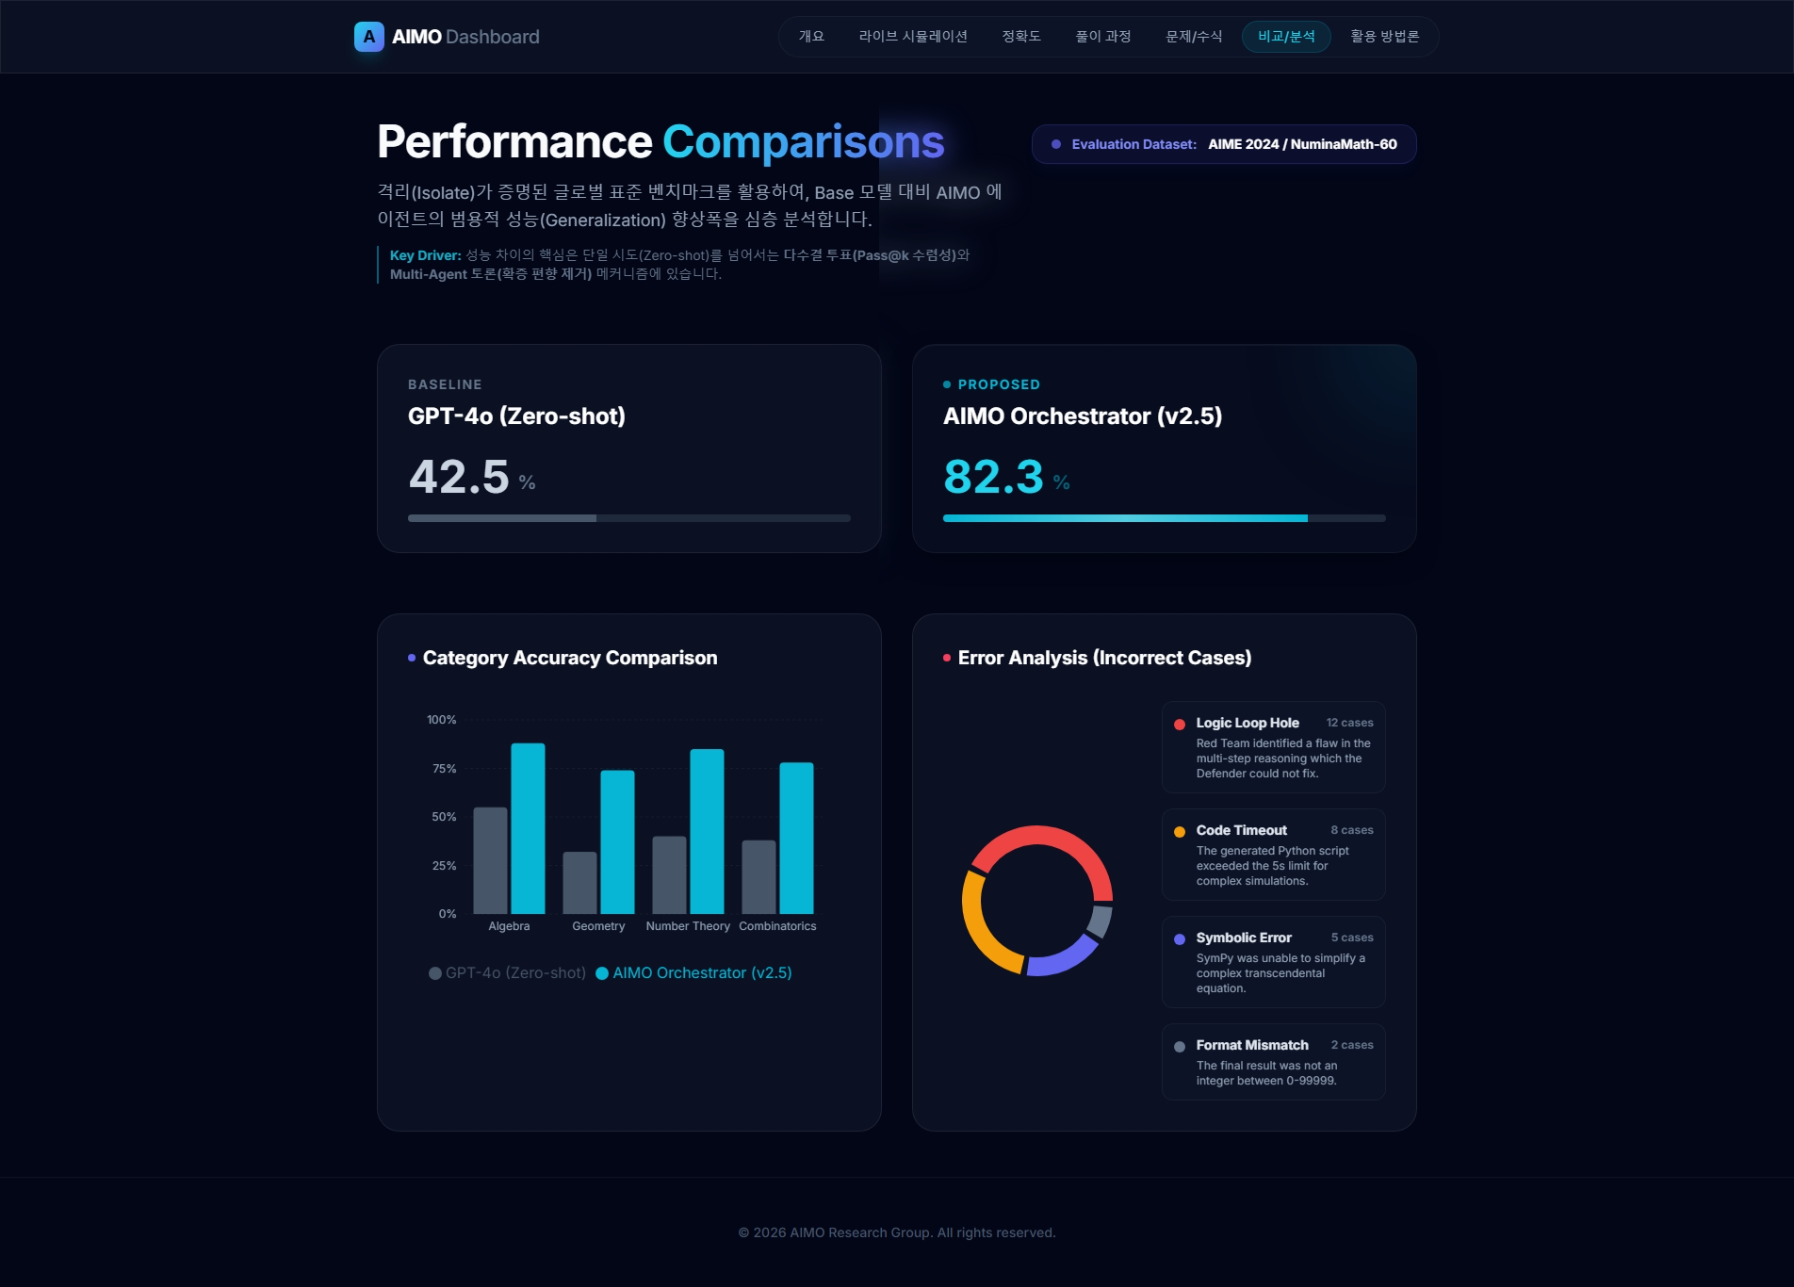
\includegraphics[width=0.95\textwidth]{dashboard_comparison.png}
\caption{Proposed OMI 오케스트레이터 파이프라인과 GPT-4o 베이스라인 간의 최종 수학 해결 성능 비교 화면}
\label{fig:dashboard_comparison}
\end{figure}

이 모든 프로세스는 Python 기반의 고성능 웹 프레임워크인 \textbf{FastAPI} 위에서 비동기(Asynchronous) 마이크로서비스(`\texttt{/solve}' 엔드포인트)로 제공됩니다.

\subsection{교육용 투명 대시보드 구현 (Glass-box UI/UX)}

아무리 뛰어난 추론 능력을 가진 AI라 할지라도, 그 과정이 철저히 감춰진 `블랙박스(Black-box)'라면 교육 도구로서의 가치는 반감됩니다. 학생들은 AI가 툭 던져준 정답을 외우는 것이 아니라, AI가 \textbf{어떠한 논리적 근거로 공식을 선택하고, 코드를 어떻게 작성하며, 실수를 어떻게 교정하는지} 그 흐름을 관찰해야 합니다.

이를 위해 Vite와 React 기반으로 개발된 AIMO 대시보드는 백엔드의 5단계 파이프라인의 실시간 상태를 WebSocket 및 Server-Sent Events(SSE)를 통해 스트리밍 받아 시각화합니다. 백엔드의 분석 상태 변화가 실시간으로 프론트엔드 UI 컴포넌트로 플로우되어 투명하게 노출되는 구체적 구조는 그림 \ref{fig:dashboard_streaming}와 같습니다.

\begin{figure}[htbp]
\centering
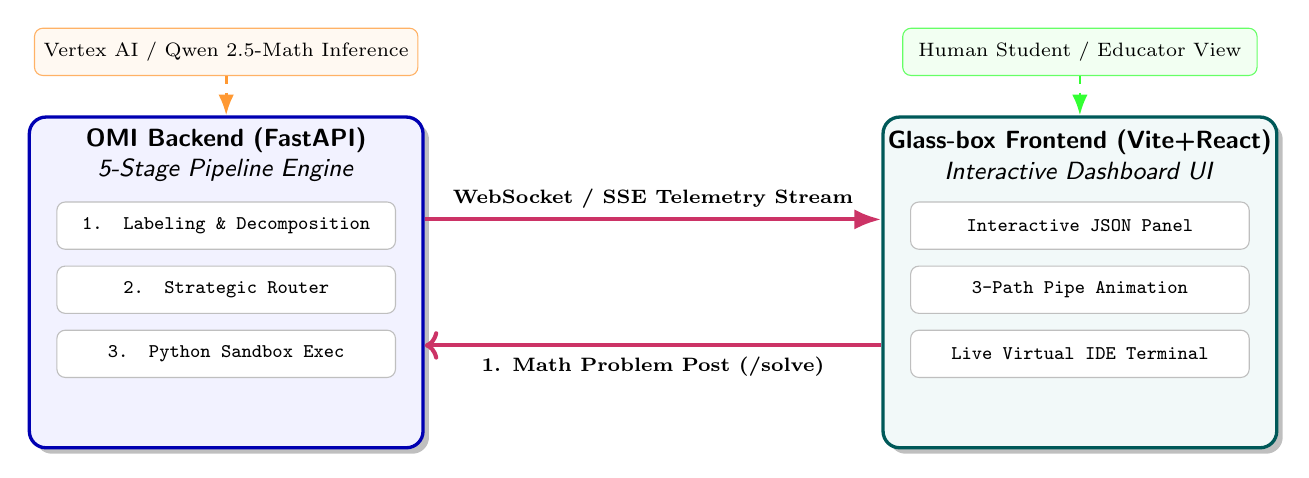
\begin{tikzpicture}[
    node distance=1.5cm and 1.5cm,
    every node/.style={font=\small\sffamily, align=center},
    backend/.style={rectangle, draw=blue!70!black, fill=blue!5, rounded corners=6pt, minimum width=5cm, minimum height=4.2cm, line width=1.2pt, drop shadow},
    frontend/.style={rectangle, draw=teal!70!black, fill=teal!5, rounded corners=6pt, minimum width=5cm, minimum height=4.2cm, line width=1.2pt, drop shadow},
    arrow/.style={-Latex, line width=1.5pt, draw=purple!80},
    comp/.style={rectangle, draw=gray!50, fill=white, rounded corners=3pt, minimum width=4.3cm, minimum height=0.6cm, font=\scriptsize\ttfamily}
]

% Backend Block
\node (back) [backend] {};
\node (back_title) at ([yshift=-0.5cm]back.north) {\textbf{OMI Backend (FastAPI)} \\ \textit{\small 5-Stage Pipeline Engine}};
\node (b1) [comp] at ([yshift=-1.4cm]back.north) {1. Labeling \& Decomposition};
\node (b2) [comp, below=0.2cm of b1] {2. Strategic Router};
\node (b3) [comp, below=0.2cm of b2] {3. Python Sandbox Exec};

% Frontend Block
\node (front) [frontend, right=5.8cm of back] {};
\node (front_title) at ([yshift=-0.5cm]front.north) {\textbf{Glass-box Frontend (Vite+React)} \\ \textit{\small Interactive Dashboard UI}};
\node (f1) [comp] at ([yshift=-1.4cm]front.north) {Interactive JSON Panel};
\node (f2) [comp, below=0.2cm of f1] {3-Path Pipe Animation};
\node (f3) [comp, below=0.2cm of f2] {Live Virtual IDE Terminal};

% Connection Channels
\draw [arrow, transform canvas={yshift=0.8cm}] (back.east) -- node [above, font=\scriptsize\bfseries] {WebSocket / SSE Telemetry Stream} (front.west);
\draw [arrow, <-, transform canvas={yshift=-0.8cm}] (back.east) -- node [below, font=\scriptsize\bfseries] {1. Math Problem Post (/solve)} (front.west);

% Side badges or cards
\node (badge1) [rectangle, draw=orange!60, fill=orange!5, rounded corners=3pt, above=0.5cm of back, minimum width=4.5cm, minimum height=0.6cm, font=\scriptsize] {Vertex AI / Qwen 2.5-Math Inference};
\node (badge2) [rectangle, draw=green!60, fill=green!5, rounded corners=3pt, above=0.5cm of front, minimum width=4.5cm, minimum height=0.6cm, font=\scriptsize] {Human Student / Educator View};

\draw [arrow, dashed, draw=orange!80, line width=1pt] (badge1) -- (back);
\draw [arrow, dashed, draw=green!80, line width=1pt] (badge2) -- (front);

\end{tikzpicture}
\caption{OMI 백엔드와 Glass-box 대시보드 간의 실시간 원격 데이터 스트리밍 및 상호작용 아키텍처}
\label{fig:dashboard_streaming}
\end{figure}

그림 \ref{fig:dashboard_overview}는 실제 사용자가 처음 마주하게 되는 OMI 대시보드의 오버뷰(Overview) 화면이며, 전체 OMI 프로젝트의 목적과 실시간 API 상태, 그리고 각 핵심 파이프라인의 활성화 여부를 종합적으로 렌더링하고 있습니다.

\begin{figure}[htbp]
\centering
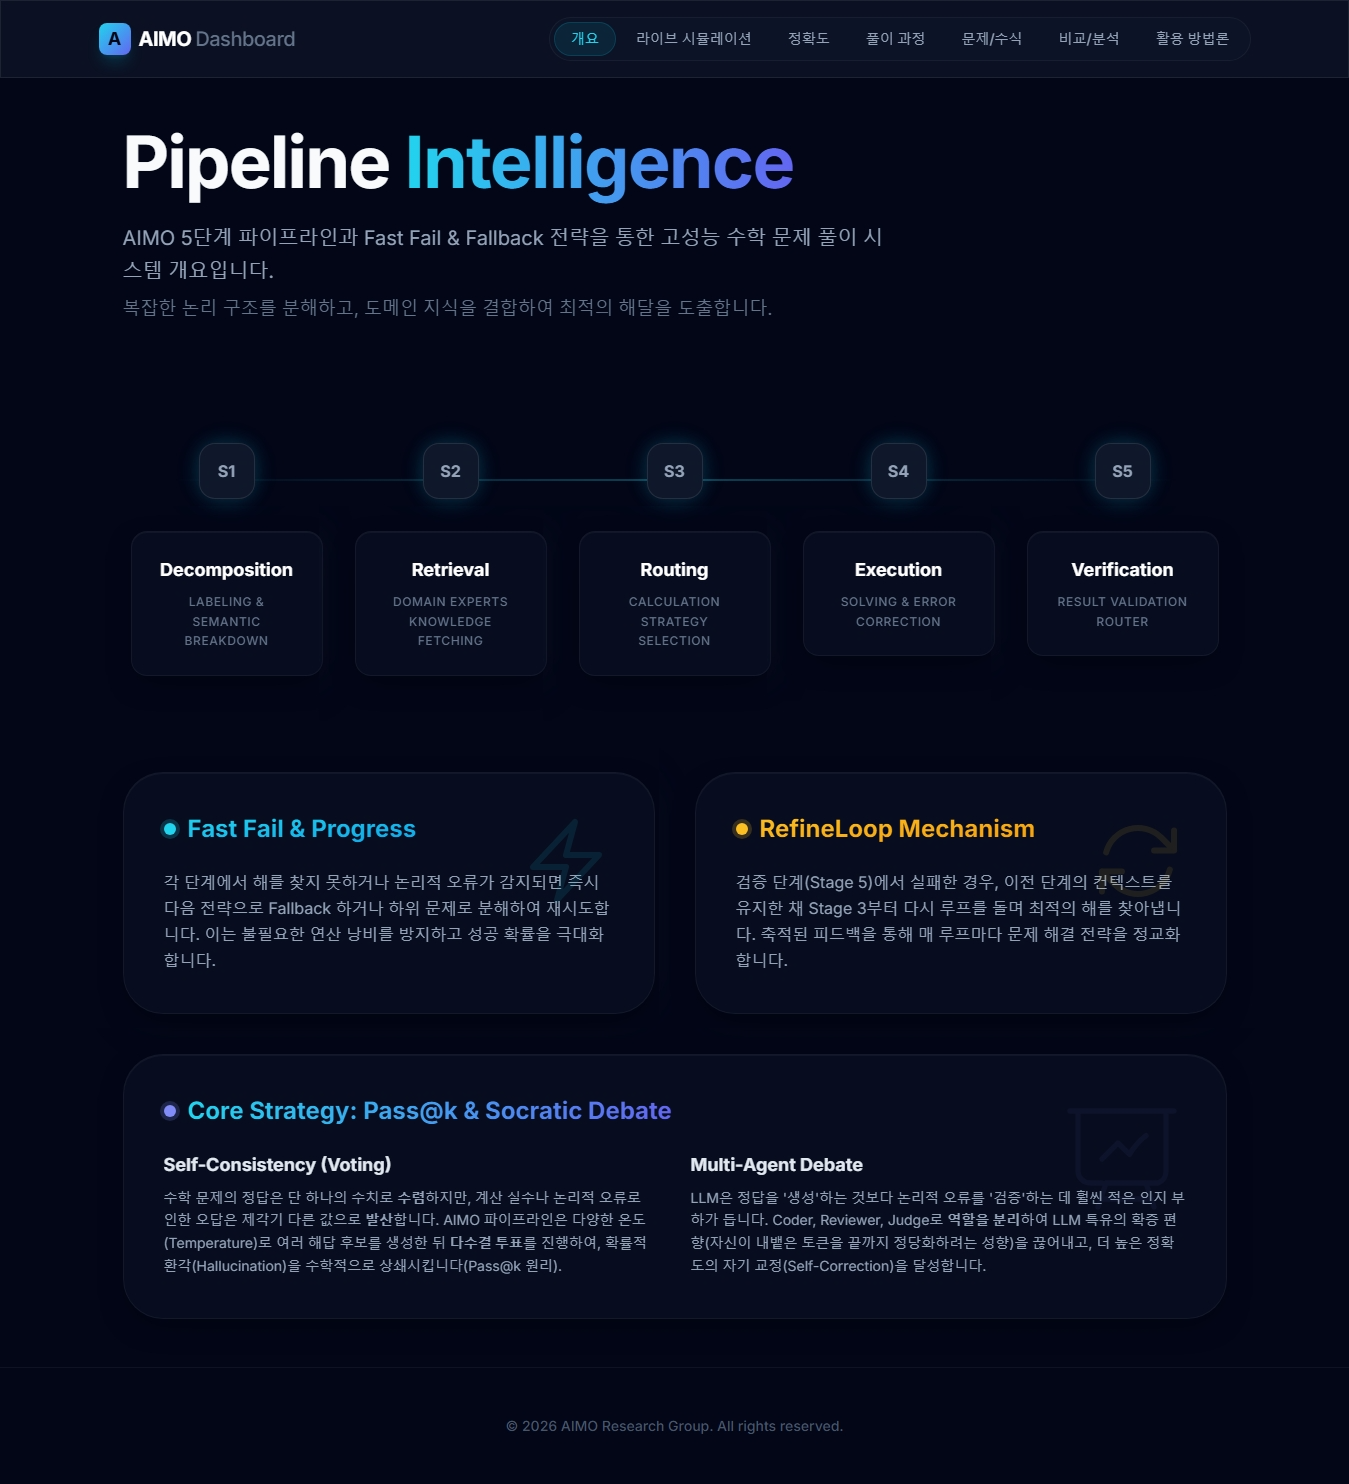
\includegraphics[width=0.95\textwidth]{dashboard_overview.png}
\caption{OMI Glass-box 대시보드 메인 오버뷰(Overview) 화면}
\label{fig:dashboard_overview}
\end{figure}

\subsubsection{XAI (설명 가능한 AI) 및 실전 구동 시나리오}
대시보드를 통해 실제 수학 문제가 풀리는 과정을 다음과 같은 `Glass-box' 시나리오로 구현했습니다.

\vspace{0.5cm}
\noindent\textbf{[User Input]:} ``$100!$ 의 끝에 연속된 0의 개수는 몇 개인가?''

\begin{enumerate}
    \item \textbf{[Stage 1: Labeling] 활성화}
    \begin{itemize}
        \item \textit{UI 표현:} 화면 중앙에 "분석 중..."이라는 스피너가 돌고, 우측 패널에 메타데이터가 JSON 형태로 타이핑됩니다.
        \item \textit{XAI 해석:} "이 문제는 \texttt{정수론(Number Theory)} 도메인이며, 핵심 타겟 변수는 $N=100$ 입니다."
    \end{itemize}
    
    \item \textbf{[Stage 2: Retrieval] 활성화}
    \begin{itemize}
        \item \textit{UI 표현:} 책장 아이콘이 반짝이며, 화면 상단에 '지식 로드 완료' 뱃지가 나타납니다.
        \item \textit{XAI 해석:} "팩토리얼의 0 개수를 구하기 위해 소인수분해 알고리즘과 \texttt{르장드르의 정리(Legendre's formula)} 템플릿을 컨텍스트에 주입했습니다."
    \end{itemize}
    
    \item \textbf{[Stage 3: Router] 활성화}
    \begin{itemize}
        \item \textit{UI 표현:} 3갈래의 파이프 애니메이션 중 가운데의 \textbf{Path B (The Theoretician)} 파이프라인으로 트래픽(빛나는 선)이 흘러갑니다.
        \item \textit{XAI 해석:} "$100!$은 천문학적으로 거대한 수이므로 시뮬레이션(Path A)으로 직접 곱하는 것은 비효율적입니다. 5의 배수를 계산하는 수학 공식을 활용하는 이론적 접근(Path B)을 선택합니다."
    \end{itemize}
    
    \item \textbf{[Stage 4: Execution] 활성화}
    \begin{itemize}
        \item \textit{UI 표현:} 다크 모드의 터미널(가상 IDE) 창이 열리며, AI가 작성하는 파이썬 코드가 한 줄씩 실시간 렌더링됩니다. `Run` 버튼 애니메이션이 작동하고 \texttt{24}라는 결과가 터미널에 출력됩니다.
    \end{itemize}
    
    \item \textbf{[Stage 5: Verification] 활성화}
    \begin{itemize}
        \item \textit{UI 표현:} 방패 모양 아이콘 안에서 체크마크가 표시됩니다.
        \item \textit{XAI 해석:} "작성된 코드의 무결성을 검증하기 위해 $N=10$으로 스케일을 줄여(Scale-Down Test) 실행한 결과 2가 도출되었으며, 이는 10!(=3,628,800)의 실제 0 개수와 일치하므로 논리가 참임을 증명합니다."
    \end{itemize}
\end{enumerate}

이러한 XAI 기반의 시각화 대시보드는 시스템이 도출한 \textbf{정답(24)보다 정답에 도달하는 논리의 흐름(사고의 지도)을 학생들에게 각인시키는 훌륭한 교육적 매개체}로 기능합니다.

그림 \ref{fig:dashboard_live}는 대시보드에서 실제로 이차방정식 문제($x^2 - 5x + 6 = 0$)를 푸는 "Live Solve" 시나리오의 실시간 입출력 화면입니다. 학생들은 자연어 문제의 입력값과 모델이 최종 검증한 수치적 출력값뿐만 아니라, 백엔드에서 시뮬레이션 경로를 타고 흘러가는 오케스트레이터의 5단계 실시간 디버그 로그와 실행 상태 폭포수(Waterfall) 궤적을 직관적으로 확인할 수 있습니다.

\begin{figure}[htbp]
\centering
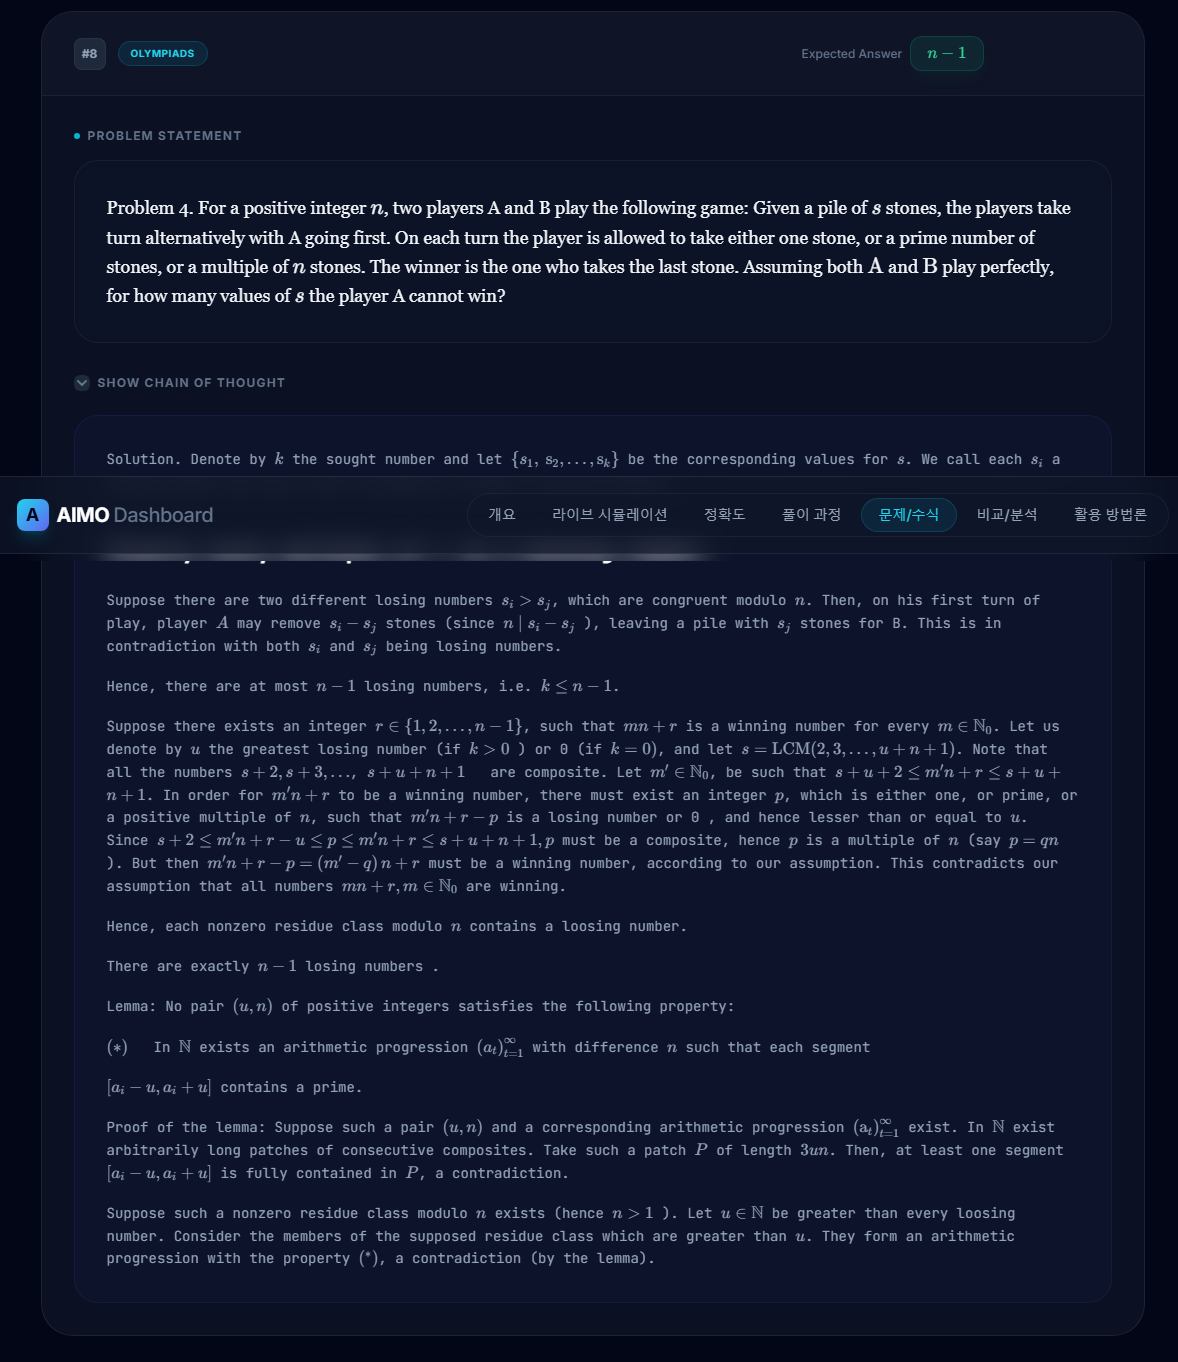
\includegraphics[width=0.95\textwidth]{dashboard_live.png}
\caption{Live Solve 페이지에서의 실제 수학 문제 입출력 및 5단계 추론 트레이스 렌더링}
\label{fig:dashboard_live}
\end{figure}

그림 \ref{fig:dashboard_xai}는 대시보드의 "풀이 과정(XAI Reasoning)" 화면으로, 기하학적 보조선이나 시각 정보가 없는 맹점 상황("눈 없는 AI")에서 수학 문제를 좌표계로 파싱하여 처리하는 단계를 시각화하고, Algebra 및 Combinatorics 등 수학 문제의 난이도별 분포 데이터를 학생들에게 제공하고 있습니다.

\begin{figure}[htbp]
\centering
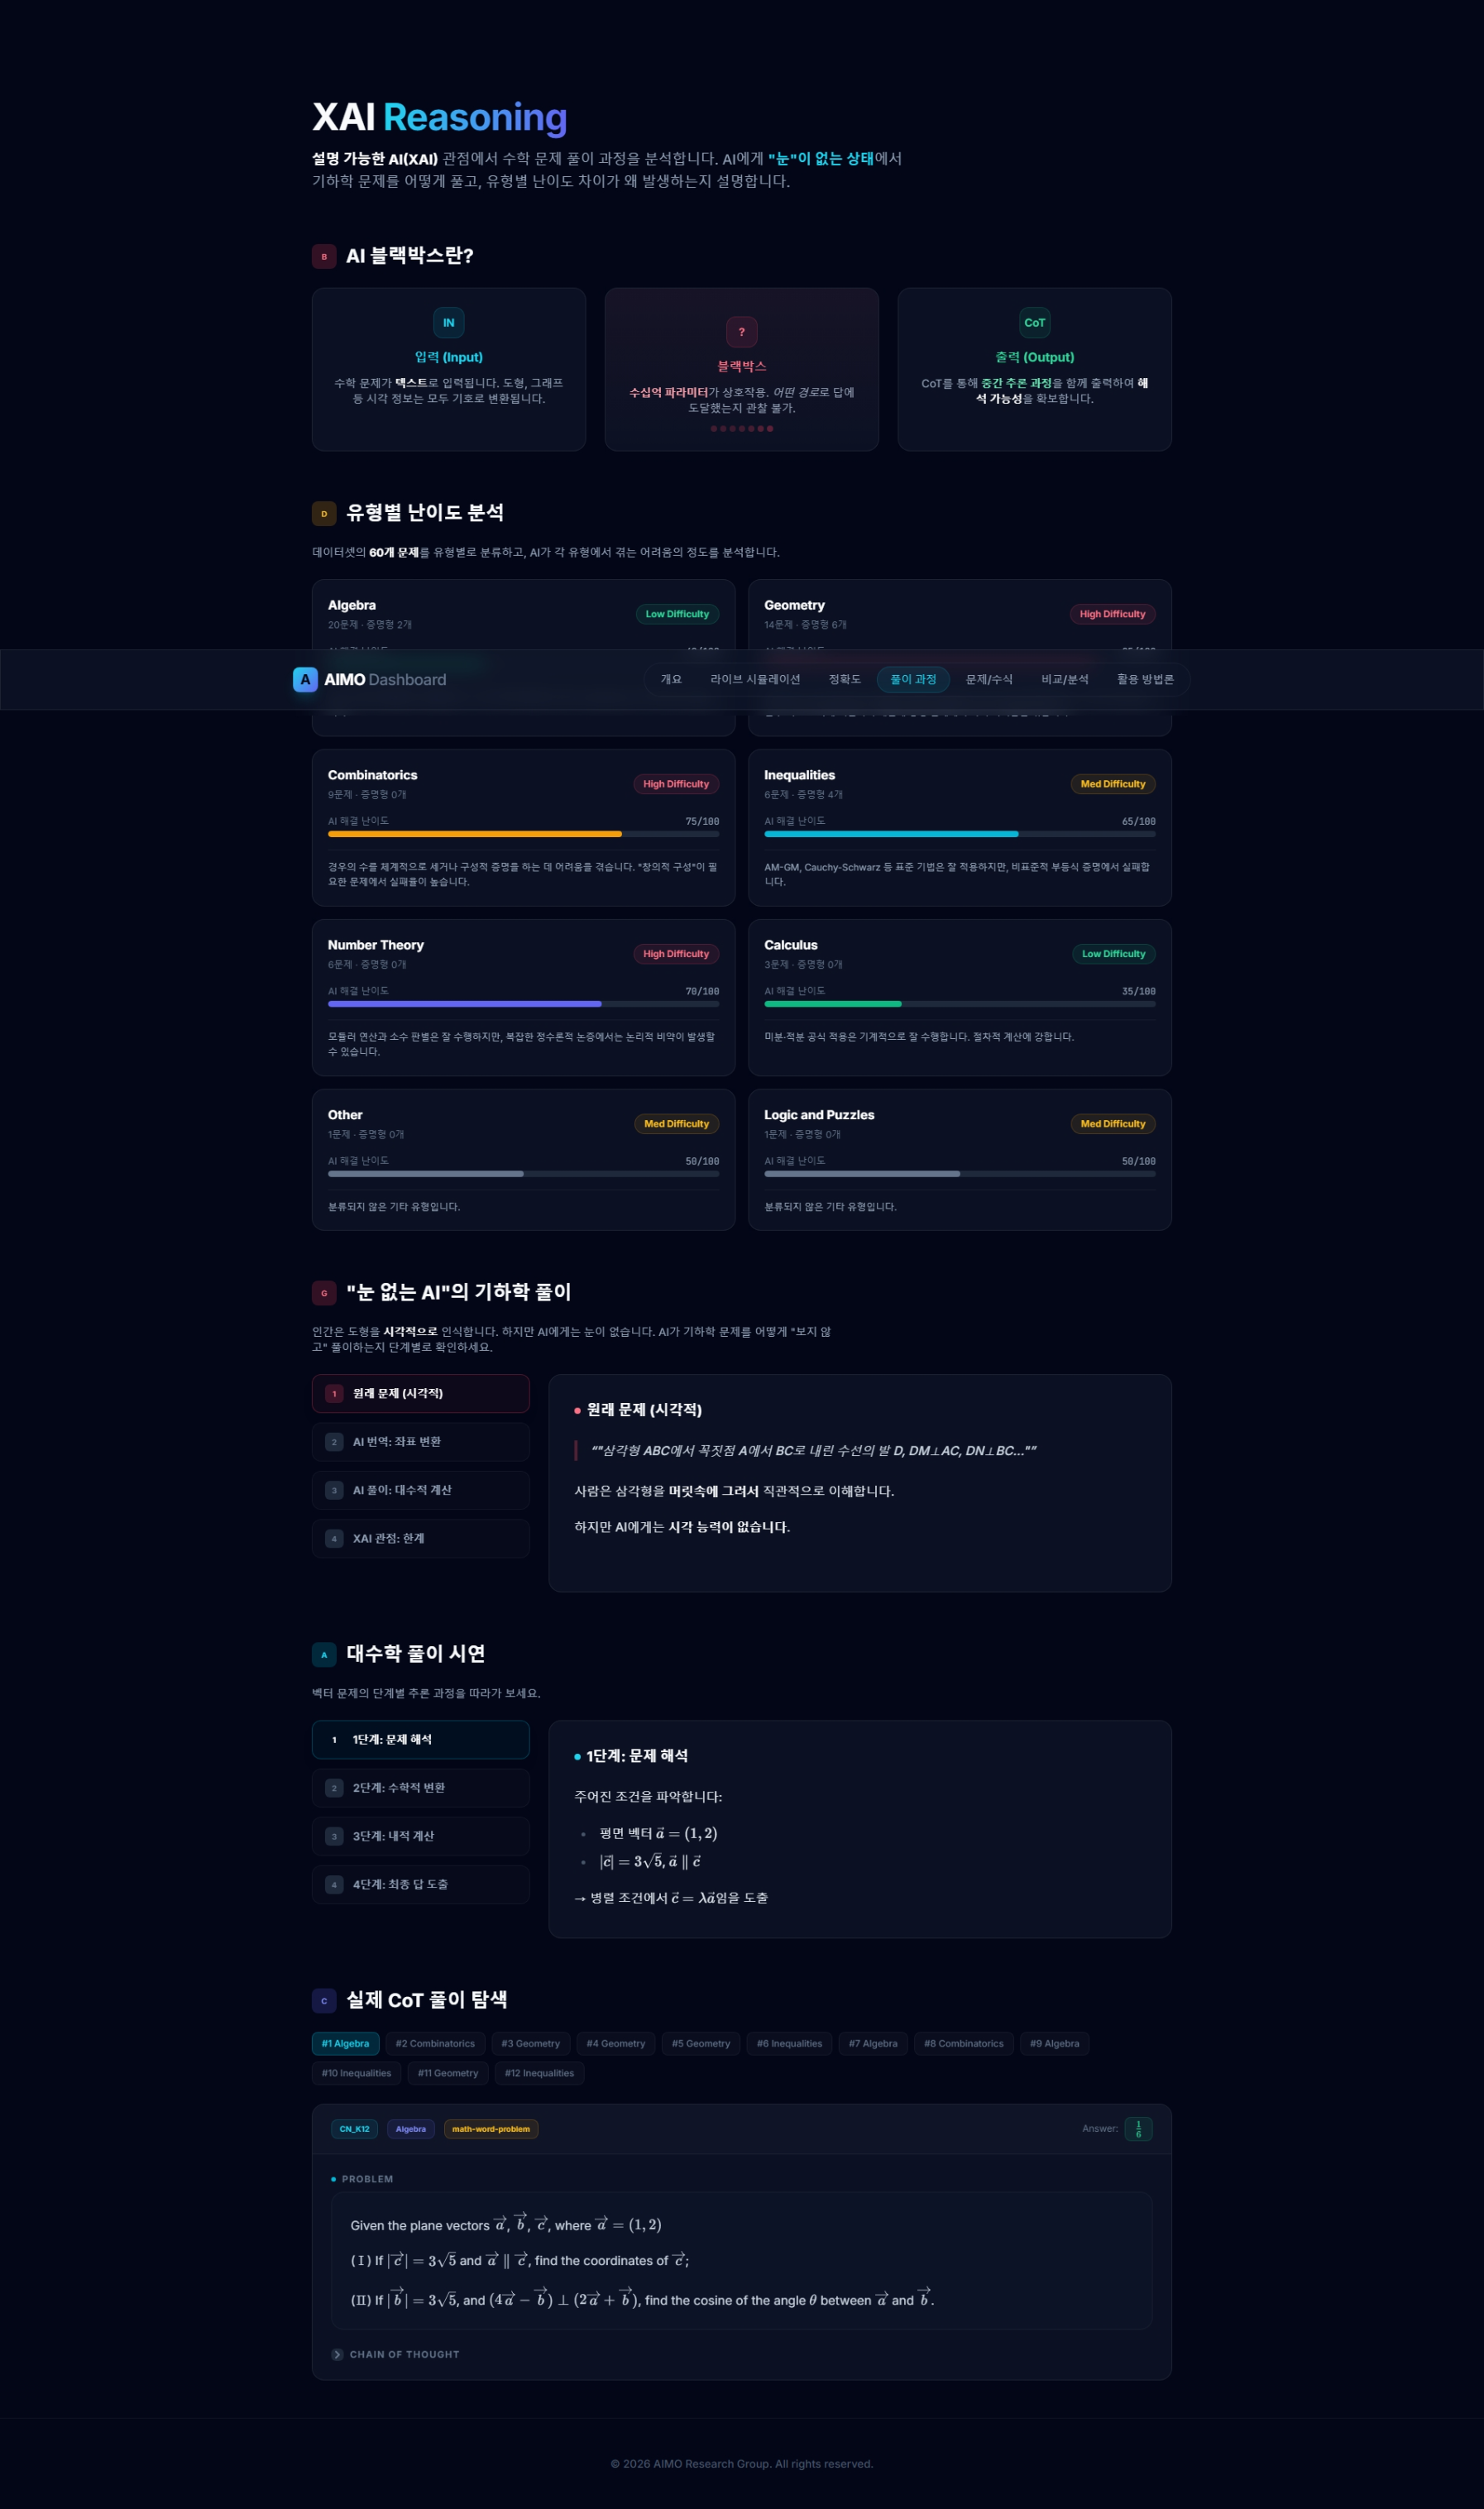
\includegraphics[width=0.95\textwidth]{dashboard_xai.png}
\caption{대시보드의 XAI Reasoning(풀이 과정) 페이지로, 유형별 난이도 분석 및 기하학/대수학 해결 메커니즘을 렌더링}
\label{fig:dashboard_xai}
\end{figure}

\newpage
\section{Conclusion (결론)}

인공지능이 인간의 지적 노동을 대체해 나가는 현시대에, 가장 복잡하고 정교한 사유가 요구되는 '수학(Mathematics)'은 LLM이 정복해야 할 최후의 보루 중 하나로 여겨졌습니다. 본 연구에서 설계하고 구현한 **OMI (Orchestrated Math Interpreter)** 시스템은, 언어 모델의 본질적 한계를 억지로 뜯어고치려 하기보다는, 그 한계를 명확히 인정하고 외부 시스템(파이썬 샌드박스)과 앙상블 체계를 통해 이를 영리하게 우회하는 '에이전트 오케스트레이션(Agentic Orchestration)'의 모범적 해답을 제시했습니다.

\subsection{연구 성과 요약}
본 연구의 핵심 성과는 크게 세 가지 축으로 요약할 수 있습니다.
첫째, 인간 수학자의 문제 해결 과정을 소프트웨어적으로 모델링한 **5단계 심층 추론 파이프라인(5-Stage Deep Reasoning Pipeline)**의 완성입니다. 단순한 질의응답 챗봇 수준을 벗어나, 도메인 분류, 지식 검색, 전략 라우팅, 실행 및 에러 정제, 최종 교차 검증이라는 체계적인 프로세스를 통해 수학 문제에 대한 극도의 논리적 강건성(Robustness)을 확보했습니다.
둘째, 데이터 오염에 대응하기 위한 **역공학 기반의 합성 데이터 엔진(Open-Reverse-Math)** 개발입니다. 정답에서 출발하여 문제를 파생시키는 이 역발상적 접근은, 모델에게 단순한 암기가 아닌 '문제를 설계하고 해체하는 메타인지'를 학습시키는 데 성공했습니다.
셋째, 백엔드의 복잡한 추론 과정을 프론트엔드로 투명하게 공개한 **Glass-box 교육용 대시보드 및 XAI**의 구현입니다. 이를 통해 AI가 정답에 도달하는 과정을 인간이 직관적으로 이해하고 통제할 수 있게 되었습니다.

\subsection{한계점 및 향후 과제 (Limitations and Future Work)}
현재 OMI 시스템은 대수학, 정수론, 이산수학과 같이 정답이 명확한 수치로 떨어지는 문제에서는 압도적인 성능을 보이나, 복잡한 기하학적 증명이나 텍스트 위주의 위상수학 문제에서는 파이썬 코드로 치환(Translate)하기 까다로운 한계가 존재합니다. 
향후 연구에서는 시각적 추론이 가능한 멀티모달(Multi-modal) VLM(Vision-Language Model)을 파이프라인에 통합하여, 도형이나 그래프 이미지를 입력받아 좌표 평면 위의 수식으로 자동 변환하는 기능을 추가할 계획입니다. 또한 본 아키텍처는 수학뿐만 아니라, 극도의 논리적 정밀함이 요구되는 법률 문서 분석 및 복잡한 소프트웨어 버그 디버깅 에이전트로 확장(Scale-out)될 수 있는 무한한 잠재력을 가지고 있습니다.
\newpage
\section{References (참고문헌)}

본 연구에서 제안한 OMI 시스템의 설계와 실험의 기초가 된 핵심 학술 문헌 및 오픈소스 기술의 출처를 APA 7판(APA 7th Edition) 규격에 맞춰 정리합니다.

\begingroup
\setlength{\parindent}{-1.5em}
\setlength{\leftskip}{1.5em}
\setlength{\parskip}{0.6em}
\setstretch{1.3} % 참고문헌 리스트의 조밀한 가독성을 위해 줄간격 조정

Chen, W., Ma, X., Wang, X., \& Cohen, W. W. (2022). Program of thoughts prompting: Disentangling computation from reasoning for numerical reasoning tasks. \textit{arXiv preprint arXiv:2211.12588}. \url{https://doi.org/10.48550/arXiv.2211.12588} \par

Gao, L., Madaan, A., Zhou, S., Alon, U., Liu, P., Yang, Y., Callan, J., \& Neubig, G. (2023). PAL: Program-aided language models. \textit{Proceedings of the 40th International Conference on Machine Learning}, 10764–10799. \url{https://proceedings.mlr.press/v202/gao23a.html} \par

Google DeepMind. (2023). \textit{Gemini: A family of highly capable multimodal models} (Technical Report). Google. \url{https://arxiv.org/abs/2312.11805} \par

Li, Y., Min, B., Zhang, Y., \& Zhang, X. (2024). \textit{NuminaMath: A diverse and high-quality dataset for mathematical reasoning} (Technical Report). Project Numina. \url{https://github.com/project-numina/numina-math} \par

Meurer, A., Smith, C. P., Paprocki, M., Čertík, O., Kirpichev, S. B., Podkalicki, M., ... \& Granger, B. E. (2017). SymPy: symbolic computing in Python. \textit{PeerJ Computer Science}, \textit{3}, e103. \url{https://doi.org/10.7717/peerj-cs.103} \par

Wang, X., Wei, J., Schuurmans, D., Le, Q., Chi, E., Narang, S., Chowdhery, A., \& Zhou, D. (2022). Self-consistency improves chain of thought reasoning in language models. \textit{Advances in Neural Information Processing Systems}, \textit{35}, 27384–27397. \url{https://arxiv.org/abs/2203.11171} \par

Wei, J., Wang, X., Schuurmans, D., Bosma, M., Ichter, B., Xia, F., Chi, E., Le, Q. V., \& Zhou, D. (2022). Chain-of-thought prompting elicits reasoning in large language models. \textit{Advances in Neural Information Processing Systems}, \textit{35}, 24824–24837. \url{https://arxiv.org/abs/2201.11903} \par

Yang, J., Yang, S., Cui, J., An, Y., Liu, C., Wang, S., Zhou, A., Lin, J., Zhang, J., \& Zhou, C. (2024). \textit{Qwen2.5-Math: Technical report} (Technical Report). Alibaba Group. \url{https://arxiv.org/abs/2409.12122} \par

\endgroup

\newpage
\section{Appendix: 핵심 용어 및 개념 사전 (Glossary)}

본 보고서에서 사용된 주요 기술적 용어와 개념들을 전공자와 비전공자 모두 명확히 이해할 수 있도록 일상적인 비유와 함께 상세히 해설합니다.

\begin{itemize}
    \item \textbf{오케스트레이션 (Orchestration)}
    \begin{itemize}
        \item \textit{개념:} 단일 AI 모델이 모든 작업을 처리하는 대신, 여러 전문화된 에이전트와 도구들의 작업 순서와 상호작용을 중앙에서 지휘하고 조율하는 시스템 아키텍처.
        \item \textit{비유:} 교향악단의 지휘자(Orchestrator). 바이올린(언어 능력)과 팀파니(연산 능력)가 제각각 연주하지 않도록, 악보(프롬프트와 파이프라인)에 맞춰 각자가 정확한 타이밍에 개입하게 만드는 역할을 합니다.
    \end{itemize}
    
    \item \textbf{TIR (Tool-Integrated Reasoning, 도구 결합 추론)}
    \begin{itemize}
        \item \textit{개념:} 언어 모델이 자연어로만 추론을 끝내지 않고, 파이썬 코드 실행기나 심볼릭 계산기(\texttt{SymPy}), 혹은 웹 브라우저와 같은 외부 도구(Tool)를 직접 호출하여 얻은 결과값을 다시 자신의 추론 문맥에 통합하는 기술.
        \item \textit{비유:} 머릿속으로만 8자리 곱셈을 하려 끙끙대는 대신, 주머니에서 공학용 계산기를 꺼내 두드려 본 뒤 그 액정 화면의 결과를 답안지에 적어내는 똑똑한 수험생의 행동과 같습니다.
    \end{itemize}
    
    \item \textbf{다수결 투표 (Majority Voting) 와 Pass@$k$}
    \begin{itemize}
        \item \textit{개념:} LLM의 생성 과정에 내재된 확률적 다양성을 활용하는 앙상블 기법. $k$번 독립적으로 생성(Pass@$k$)한 결과들 중 가장 높은 빈도로 등장한 값을 최종 정답으로 채택합니다.
        \item \textit{비유:} "백지장도 백 번 맞들면 낫다." 한 명의 덜렁대는 학생에게 똑같은 문제를 100번 풀게 시킵니다. 계산 실수를 하면 100번 모두 각각 엉뚱한 수치로 발산하지만, 논리가 맞았다면 무조건 하나의 올바른 정답으로 수렴합니다. 따라서 가장 많이 나온 답을 고르면 계산 실수를 완벽히 솎아낼 수 있습니다.
    \end{itemize}

    \item \textbf{Scale-Down Test (축소 검증)}
    \begin{itemize}
        \item \textit{개념:} 문제의 목표 파라미터가 천문학적으로 커서($N=10^{100}$) 직접적인 검증이 불가능할 때, 파라미터를 극단적으로 축소하여($N=3$) 해당 알고리즘이나 수식의 참/거짓 유무를 빠르게 가늠하는 디버깅 기법.
        \item \textit{비유:} 수백만 톤의 하중을 견뎌야 하는 거대한 금문교를 실제 크기로 짓기 전에, 동일한 비율로 축소한 미니어처 다리를 풍동 실험실에 넣어보고 무너지지 않는지 미리 테스트하는 물리적 검증 과정과 동일합니다.
    \end{itemize}

    \item \textbf{확증 편향 (Confirmation Bias in Auto-regressive Models)}
    \begin{itemize}
        \item \textit{개념:} LLM이 왼쪽에서 오른쪽으로(Left-to-Right) 단어를 예측해 나갈 때, 한 번 오답 토큰을 생성하고 나면 그 오답이 뒤따르는 문맥에 조건부 확률(Conditioning)로 묶여, 스스로 틀렸음을 인지하지 못하고 끝까지 오답을 정당화하려는 현상.
        \item \textit{비유:} 거짓말을 한 번 하고 나면 그 거짓말을 덮기 위해 계속해서 더 큰 거짓말을 지어내며, 절대 자신이 틀렸다고 인정하지 않는 고집쟁이의 모습에 비유할 수 있습니다. (OMI는 백지상태의 Reviewer 에이전트를 투입해 이를 교정합니다.)
    \end{itemize}

    \item \textbf{역공학 데이터 생성 (Reverse Engineering Data Generation)}
    \begin{itemize}
        \item \textit{개념:} "문제 $\rightarrow$ 정답"의 일반적인 데이터 생성 패러다임을 뒤집어, 미리 목표 정답을 확정지은 후 이 정답을 해(Root)로 가지는 복잡한 수학적 구조(다항식, 기하학 모델)를 구축하고, 이를 다시 자연어로 감추어(Obfuscation) 무오류의 문제를 대량 합성하는 기법.
        \item \textit{비유:} 아주 복잡한 미로 찾기 퍼즐 책을 만들 때, 입구에서 출발하며 길을 그리는 대신 출구(정답)에서부터 연필을 대고 거꾸로 미로를 그려 나가는 방식입니다. 이 방법을 쓰면 절대 출구가 없는 엉터리 미로가 만들어지지 않습니다.
    \end{itemize}

    \item \textbf{XAI (Explainable AI, 설명 가능한 인공지능)}
    \begin{itemize}
        \item \textit{개념:} 딥러닝과 신경망의 예측 결과가 어떠한 수학적, 논리적 근거에 의해 도출되었는지 그 의사결정 과정을 인간이 이해할 수 있는 자연어와 시각적 요소로 풀어서 설명해 주는 기술.
        \item \textit{비유:} "정답은 4번입니다"라고만 말하고 입을 닫는 무뚝뚝한 컴퓨터가 아니라, "이 문제를 시뮬레이션으로 풀려고 했으나 메모리가 초과될 것 같아, 제가 이러이러한 수학 공식을 이용한 파이썬 코드를 짰고, 그래서 이런 결과가 나왔습니다"라고 친절하게 풀이 과정을 해설해 주는 일타 강사의 해설지와 같습니다.
    \end{itemize}
\end{itemize}


\end{document}
